\documentclass{article}

\usepackage[margin=1em]{geometry}
\usepackage{subcaption}
\usepackage{tikz}

\usepackage{amssymb}

\title{Computations of path overheads w.r.t. Manhattan Distance}
\date{}

\def\vspacing{50pt}
\tikzstyle{count}=[scale=1.5]

\begin{document}
	\maketitle

	\section{Source {\tt XZZ}@(0,0,0), Manhattan Distance $= 1$, positive octant}
	\begin{figure}[h!]
		% Target XZZ
		\begin{subfigure}{0.16\textwidth}
			\centering
			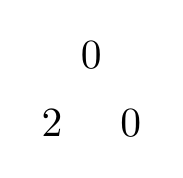
\begin{tikzpicture}
				\node[count] at (0:0) {2};
				\node[count] at (0:1) {0};
				\node[count] at (60:1) {0};
			\end{tikzpicture}
			\caption{Target {\tt XZZ}}
		\end{subfigure}
		% Target ZXZ
		\begin{subfigure}{0.16\textwidth}
			\centering
			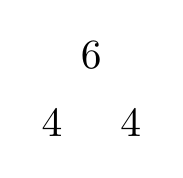
\begin{tikzpicture}
				\node[count] at (0:0) {4};
				\node[count] at (0:1) {4};
				\node[count] at (60:1) {6};
			\end{tikzpicture}
			\caption{Target {\tt ZXZ}}
		\end{subfigure}
		% Target ZZX
		\begin{subfigure}{0.16\textwidth}
			\centering
			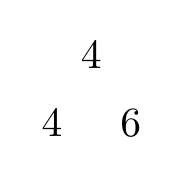
\begin{tikzpicture}
				\node[count] at (0:0) {4};
				\node[count] at (0:1) {6};
				\node[count] at (60:1) {4};
			\end{tikzpicture}
			\caption{Target {\tt ZZX}}
		\end{subfigure}
		% Target ZXX
		\begin{subfigure}{0.16\textwidth}
			\centering
			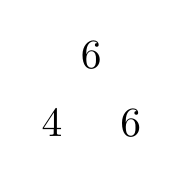
\begin{tikzpicture}
				\node[count] at (0:0) {4};
				\node[count] at (0:1) {6};
				\node[count] at (60:1) {6};
			\end{tikzpicture}
			\caption{Target {\tt ZXX}}
		\end{subfigure}
		% Target XZX
		\begin{subfigure}{0.16\textwidth}
			\centering
			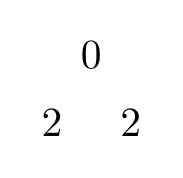
\begin{tikzpicture}
				\node[count] at (0:0) {2};
				\node[count] at (0:1) {2};
				\node[count] at (60:1) {0};
			\end{tikzpicture}
			\caption{Target {\tt XZX}}
		\end{subfigure}
		% Target XXZ
		\begin{subfigure}{0.16\textwidth}
			\centering
			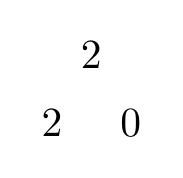
\begin{tikzpicture}
				\node[count] at (0:0) {2};
				\node[count] at (0:1) {0};
				\node[count] at (60:1) {2};
			\end{tikzpicture}
			\caption{Target {\tt XXZ}}
		\end{subfigure}
	\end{figure}


	\section{Source {\tt XZZ}@(0,0,0), Manhattan Distance $= 2$, positive octant}

	\begin{figure}[h!]
		% Target XZZ
		\begin{subfigure}{0.33\textwidth}
			\centering
			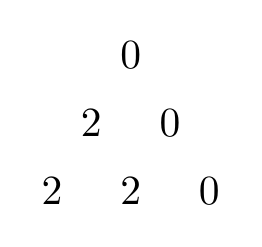
\begin{tikzpicture}
				\node[count] at (0:0) {2};
				\node[count] at (0:1) {2};
				\node[count] at (0:2) {0};
				\node[count] at ([shift={(60:1)}] 0:0) {2};
				\node[count] at ([shift={(60:1)}] 0:1) {0};
				\node[count] at ([shift={(60:2)}] 0:0) {0};
			\end{tikzpicture}
			\caption{Target {\tt XZZ}}
			\vspace*{\vspacing}
		\end{subfigure}
		% Target ZXZ
		\begin{subfigure}{0.33\textwidth}
			\centering
			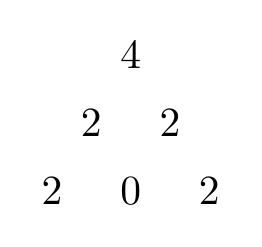
\begin{tikzpicture}
				\node[count] at (0:0) {2};
				\node[count] at (0:1) {0};
				\node[count] at (0:2) {2};
				\node[count] at ([shift={(60:1)}] 0:0) {2};
				\node[count] at ([shift={(60:1)}] 0:1) {2};
				\node[count] at ([shift={(60:2)}] 0:0) {4};
			\end{tikzpicture}
			\caption{Target {\tt ZXZ}}
			\vspace*{\vspacing}
		\end{subfigure}
		% Target ZZX
		\begin{subfigure}{0.33\textwidth}
			\centering
			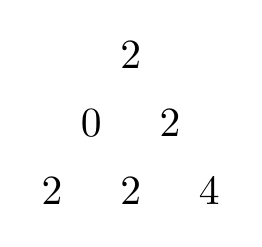
\begin{tikzpicture}
				\node[count] at (0:0) {2};
				\node[count] at (0:1) {2};
				\node[count] at (0:2) {4};
				\node[count] at ([shift={(60:1)}] 0:0) {0};
				\node[count] at ([shift={(60:1)}] 0:1) {2};
				\node[count] at ([shift={(60:2)}] 0:0) {2};
			\end{tikzpicture}
			\caption{Target {\tt ZZX}}
			\vspace*{\vspacing}
		\end{subfigure}
		% Target ZXX
		\begin{subfigure}{0.33\textwidth}
			\centering
			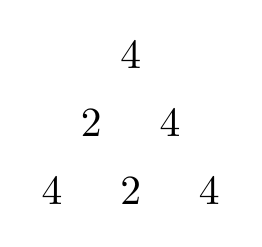
\begin{tikzpicture}
				\node[count] at (0:0) {4};
				\node[count] at (0:1) {2};
				\node[count] at (0:2) {4};
				\node[count] at ([shift={(60:1)}] 0:0) {2};
				\node[count] at ([shift={(60:1)}] 0:1) {4};
				\node[count] at ([shift={(60:2)}] 0:0) {4};
			\end{tikzpicture}
			\caption{Target {\tt ZXX}}
		\end{subfigure}
		% Target XZX
		\begin{subfigure}{0.33\textwidth}
			\centering
			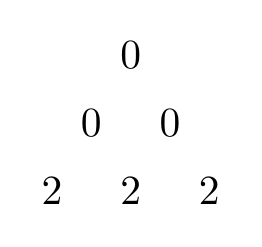
\begin{tikzpicture}
				\node[count] at (0:0) {2};
				\node[count] at (0:1) {2};
				\node[count] at (0:2) {2};
				\node[count] at ([shift={(60:1)}] 0:0) {0};
				\node[count] at ([shift={(60:1)}] 0:1) {0};
				\node[count] at ([shift={(60:2)}] 0:0) {0};
			\end{tikzpicture}
			\caption{Target {\tt XZX}}
		\end{subfigure}
		% Target XXZ
		\begin{subfigure}{0.33\textwidth}
			\centering
			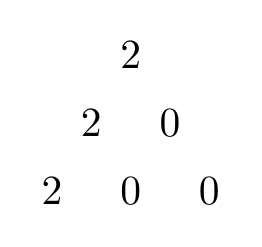
\begin{tikzpicture}
				\node[count] at (0:0) {2};
				\node[count] at (0:1) {0};
				\node[count] at (0:2) {0};
				\node[count] at ([shift={(60:1)}] 0:0) {2};
				\node[count] at ([shift={(60:1)}] 0:1) {0};
				\node[count] at ([shift={(60:2)}] 0:0) {2};
			\end{tikzpicture}
			\caption{Target {\tt XXZ}}
		\end{subfigure}
	\end{figure}
	\newpage

	\section{Source {\tt XZZ}@(0,0,0), Manhattan Distance $\geqslant 3$, positive octant}

	\begin{figure}[h!]
		% Target XZZ
		\begin{subfigure}{0.5\textwidth}
			\centering
			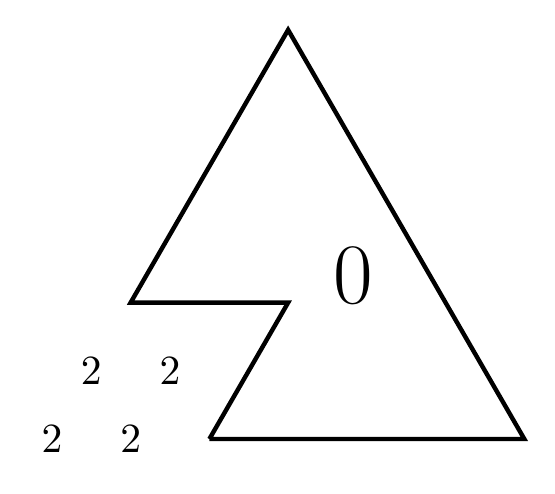
\begin{tikzpicture}
				\draw[black, ultra thick] (0:2) -- ++(0:4) -- ++(120:6) -- ++(240:4) -- ++(0:2) -- ++(240:2);
				\node[count] at (0:0) {2};
				\node[count] at (0:1) {2};
				\node[count] at ([shift={(60:1)}] 0:0) {2};
				\node[count] at ([shift={(60:1)}] 0:1) {2};
				\node[count] at ([shift={(60:2)}] 7:2.85) {\huge 0};
			\end{tikzpicture}
			\caption{Target {\tt XZZ}}
			\vspace*{\vspacing}
		\end{subfigure}
		% Target ZXX
		\begin{subfigure}{0.5\textwidth}
			\centering
			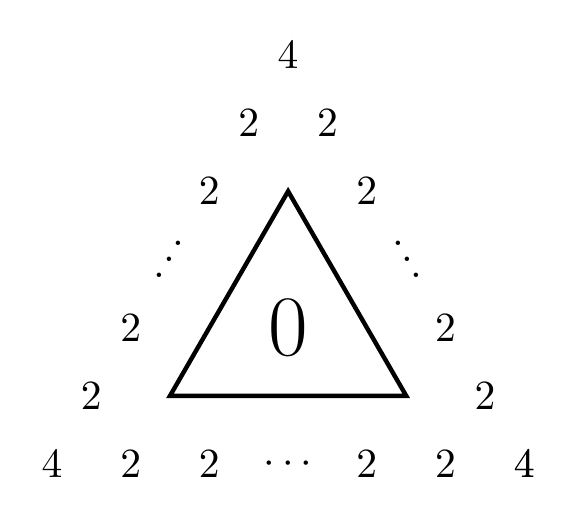
\begin{tikzpicture}
				\draw[black, ultra thick] ([shift={(60:1)}] 0:1) -- ++(0:3) -- ++(120:3) -- cycle;
				\node[count] at (0:0) {4};
				\node[count] at (0:1) {2};
				\node[count] at (0:2) {2};
				\node[count] at (0:3) {$\cdots$};
				\node[count] at (0:4) {2};
				\node[count] at (0:5) {2};
				\node[count] at (0:6) {4};
				\node[count] at (60:1) {2};
				\node[count] at (60:2) {2};
				\node[count, rotate=60] at (60:3) {$\cdots$};
				\node[count] at (60:4) {2};
				\node[count] at (60:5) {2};
				\node[count] at ([shift={(0:6)}] 120:0) {4};
				\node[count] at ([shift={(0:6)}] 120:1) {2};
				\node[count] at ([shift={(0:6)}] 120:2) {2};
				\node[count, rotate=-60] at ([shift={(0:6)}] 120:3) {$\cdots$};
				\node[count] at ([shift={(0:6)}] 120:4) {2};
				\node[count] at ([shift={(0:6)}] 120:5) {2};
				\node[count] at ([shift={(0:6)}] 120:6) {4};
				\node[count] at ([shift={(60:2)}] 0:2) {\huge 0};
			\end{tikzpicture}
			\caption{Target {\tt ZXX}}
			\vspace*{\vspacing}
		\end{subfigure}
		% Target ZXZ
		\begin{subfigure}{0.5\textwidth}
			\centering
			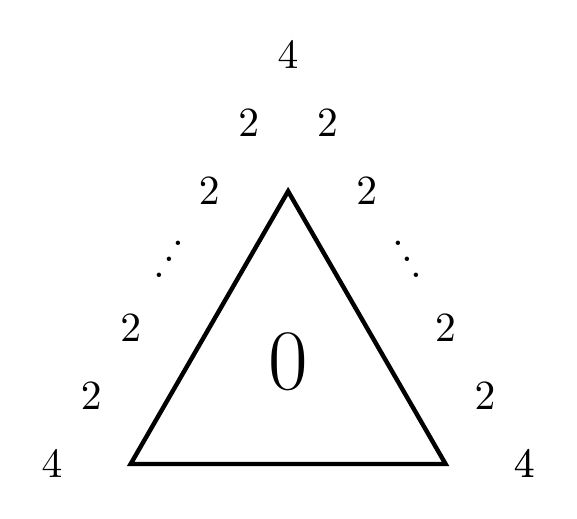
\begin{tikzpicture}
				\draw[black, ultra thick] (0:1) -- ++(0:4) -- ++(120:4) -- cycle;
				\node[count] at (0:0) {4};
				\node[count] at (0:6) {4};
				\node[count] at (60:1) {2};
				\node[count] at (60:2) {2};
				\node[count, rotate=60] at (60:3) {$\cdots$};
				\node[count] at (60:4) {2};
				\node[count] at (60:5) {2};
				\node[count] at ([shift={(0:6)}] 120:0) {4};
				\node[count] at ([shift={(0:6)}] 120:1) {2};
				\node[count] at ([shift={(0:6)}] 120:2) {2};
				\node[count, rotate=-60] at ([shift={(0:6)}] 120:3) {$\cdots$};
				\node[count] at ([shift={(0:6)}] 120:4) {2};
				\node[count] at ([shift={(0:6)}] 120:5) {2};
				\node[count] at ([shift={(0:6)}] 120:6) {4};
				\node[count] at ([shift={(60:1.5)}] 0:2.25) {\huge 0};
			\end{tikzpicture}
			\caption{Target {\tt ZXZ}}
			\vspace*{\vspacing}
		\end{subfigure}
		% Target XZX
		\begin{subfigure}{0.5\textwidth}
			\centering
			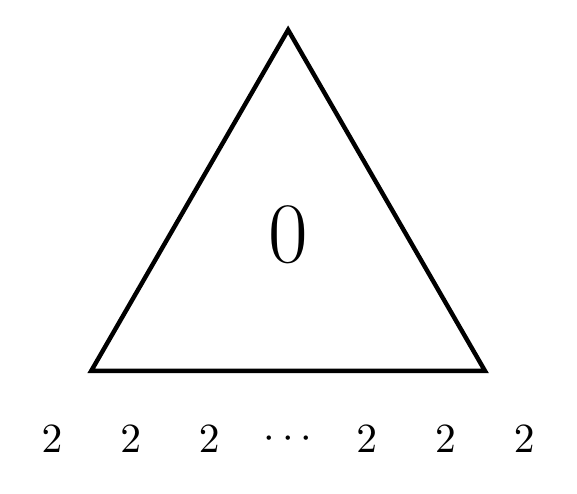
\begin{tikzpicture}
				\draw[black, ultra thick] ([shift={(60:1)}] 0:0) -- ++(0:5) -- ++(120:5) -- cycle;
				\node[count] at (0:0) {2};
				\node[count] at (0:1) {2};
				\node[count] at (0:2) {2};
				\node[count] at (0:3) {$\cdots$};
				\node[count] at (0:4) {2};
				\node[count] at (0:5) {2};
				\node[count] at (0:6) {2};
				\node[count] at ([shift={(60:3)}] 0:1.5) {\huge 0};
			\end{tikzpicture}
			\caption{Target {\tt XZX}}
			\vspace*{\vspacing}
		\end{subfigure}
		% Target ZZX
		\begin{subfigure}{0.5\textwidth}
			\centering
			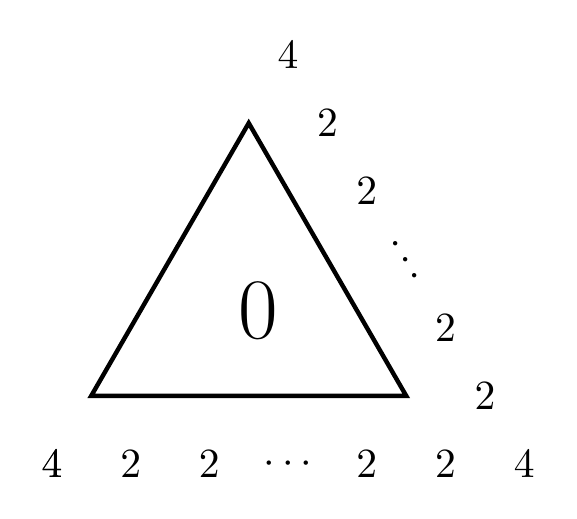
\begin{tikzpicture}
				\begin{scope}[rotate=-120]
					\draw[black, ultra thick] (0:1) -- ++(0:4) -- ++(120:4) -- cycle;
					\node[count] at (0:0) {4};
					\node[count] at (0:6) {4};
					\node[count] at (60:1) {2};
					\node[count] at (60:2) {2};
					\node[count, rotate=120] at (60:3) {$\cdots$};
					\node[count] at (60:4) {2};
					\node[count] at (60:5) {2};
					\node[count] at ([shift={(0:6)}] 120:0) {4};
					\node[count] at ([shift={(0:6)}] 120:1) {2};
					\node[count] at ([shift={(0:6)}] 120:2) {2};
					\node[count] at ([shift={(0:6)}] 120:3) {$\cdots$};
					\node[count] at ([shift={(0:6)}] 120:4) {2};
					\node[count] at ([shift={(0:6)}] 120:5) {2};
					\node[count] at ([shift={(0:6)}] 120:6) {4};
					\node[count] at ([shift={(60:1.5)}] 0:2.25) {\huge 0};
				\end{scope}
			\end{tikzpicture}
			\caption{Target {\tt ZZX}}
		\end{subfigure}
		% Target XXZ
		\begin{subfigure}{0.5\textwidth}
			\centering
			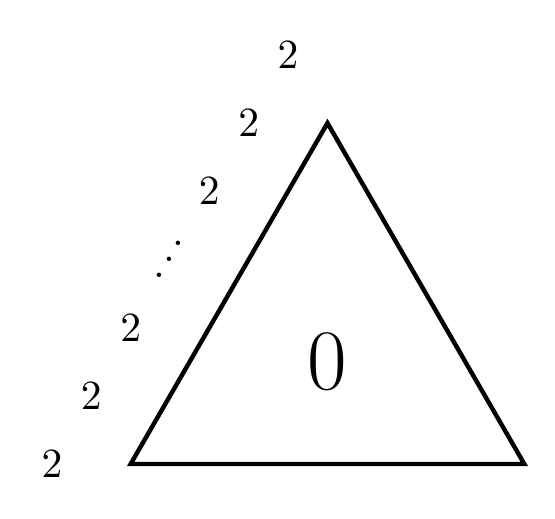
\begin{tikzpicture}
				\begin{scope}[rotate=-120]
					\draw[black, ultra thick] ([shift={(60:1)}] 0:0) -- ++(0:5) -- ++(120:5) -- cycle;
					\node[count] at (0:0) {2};
					\node[count] at (0:1) {2};
					\node[count] at (0:2) {2};
					\node[count, rotate=60] at (0:3) {$\cdots$};
					\node[count] at (0:4) {2};
					\node[count] at (0:5) {2};
					\node[count] at (0:6) {2};
					\node[count] at ([shift={(60:2.75)}] 0:1.75) {\huge 0};
				\end{scope}
			\end{tikzpicture}
			\caption{Target {\tt XXZ}}
		\end{subfigure}
	\end{figure}
\end{document}